\documentclass{article} % For LaTeX2e
\usepackage{iclr2026_conference,times}

% Optional math commands from https://github.com/goodfeli/dlbook_notation.
\input{math_commands.tex}

\usepackage{hyperref}
\usepackage{url}
\usepackage{booktabs}       % professional-quality tables
\usepackage{amsfonts}       % blackboard math symbols
\usepackage{nicefrac}       % compact symbols for 1/2, etc.
\usepackage{microtype}      % microtypography
\usepackage{xcolor}         % colors

\usepackage{wrapfig}
\usepackage{graphicx}
\usepackage{tcolorbox}
\usepackage{amsmath}
\usepackage{tabularx}

\newtcolorbox{insights}[1][]{%
    colback=blue!5!white, % Light blue background color of the box
    colframe=blue!75!black, % Darker blue border color of the box
    sharp corners, % Makes the corners of the box sharp
    toprule=0pt, % Remove top border
    bottomrule=0pt, % Remove bottom border
    leftrule=1.2pt, % Keep left border
    rightrule=1.2pt, % Keep right border
    #1 % Additional options
}

\setlength{\parskip}{2.5pt plus3pt minus2.5pt}
% 1.2pt：基础段落间距为 1.2 点（约 0.42 毫米）。
% plus3pt：允许 LaTeX 在排版需要时增加最多 3pt 的弹性间距（例如避免页面底部留白过多）。
% minus2.5pt：允许 LaTeX 在排版需要时减少最多 2.5pt 的弹性间距（例如避免内容被截断）。
% \setlength{\textfloatsep}{3pt plus2pt minus2pt} % 顶部/底部浮动体
% \setlength{\intextsep}{3pt plus2pt minus2pt}      % 中间浮动体
% 减少图表与上下文的间距（例如设为 10pt + 弹性值）

% 调整图片标题与内容的间距
% \setlength{\abovecaptionskip}{-10pt}  % 标题上方间距
% \setlength{\belowcaptionskip}{-10pt}   % 标题下方间距

% % 调整表格标题与内容的间距（表格标题通常在表格上方）
% \setlength{\abovecaptionskip}{-10pt}   % 表格标题上方间距
% \setlength{\belowcaptionskip}{-10pt}   % 表格标题下方间距

\title{Will LLMs Scaling Hit the Wall? Breaking Barriers via Distributed Resources on Massive Edge Devices}

% Authors must not appear in the submitted version. They should be hidden
% as long as the \iclrfinalcopy macro remains commented out below.
% Non-anonymous submissions will be rejected without review.

\author{Tao Shen$^{1,}$\thanks{Equal contribution}, Didi Zhu$^{1,}$\footnotemark[1], Ziyu Zhao$^{1,}$\footnotemark[1], Zexi Li$^{1,}$\thanks{Corresponding author}, Chao Wu$^{2,}$\footnotemark[2], Fei Wu$^{1,}$\footnotemark[2] \\
$^{1}$College of Computer Science and Technology, Zhejiang University, China \\
$^{2}$School of Public Affairs, Zhejiang University, China \\
\texttt{\{tao.shen, didi.zhu, ziyuzhao.cs, zexi.li, chao.wu, wufei\}@zju.edu.cn}}

% The \author macro works with any number of authors. There are two commands
% used to separate the names and addresses of multiple authors: \And and \AND.
%
% Using \And between authors leaves it to \LaTeX{} to determine where to break
% the lines. Using \AND forces a linebreak at that point. So, if \LaTeX{}
% puts 3 of 4 authors names on the first line, and the last on the second
% line, try using \AND instead of \And before the third author name.

\newcommand{\fix}{\marginpar{FIX}}
\newcommand{\new}{\marginpar{NEW}}

% \iclrfinalcopy % Uncomment for camera-ready version, but NOT for submission.
\begin{document}


\maketitle

\begin{abstract}
The remarkable success of foundation models has been driven by scaling laws, demonstrating that model performance improves predictably with increased \textit{training data} and \textit{model size}. 
However, this scaling trajectory faces two critical challenges: the exhaustion of high-quality public data, and the prohibitive computational power required for larger models, which have been monopolized by tech giants. 
These two bottlenecks pose significant obstacles to the further development of AI.
In this position paper, we argue that leveraging massive distributed edge devices can break through these barriers. 
We reveal the vast untapped potential of data and computational resources on massive edge devices, and review recent technical advancements in distributed/federated learning that make this new paradigm viable.
Our analysis suggests that by collaborating on edge devices, everyone can participate in training large language models with small edge devices.
This paradigm shift towards distributed training on edge has the potential to democratize AI development and foster a more inclusive AI community. 
The project page is available at \url{https://tao-shen.github.io/Distributed-LLM-Edges/}
\end{abstract}

\section{Introduction}

\textbf{Scaling laws} \citep{kaplan2020scaling,hoffmann2022training} have been fundamental to the remarkable success of foundation models, demonstrating a predictable relationship between performance and the expansion of model parameters and training data. These laws have guided the development of increasingly powerful models, from BERT \citep{devlin2018bert} to GPT-4 \citep{openai2023gpt4}, showing that performance improvements can be achieved through systematic scaling of both model size and training data \citep{brown2020language,chowdhery2022palm}. However, the continued application of these scaling laws requires ever-increasing amounts of data and computational resources, pushing the boundaries of what is currently feasible \citep{patterson2021carbon}. 



\textbf{Public data} has been the primary \textit{fuel} driving AI development forward. 
This field has witnessed an exponential growth in data requirements, from the early success of MNIST \citep{lecun1998mnist} with its 70,000 handwritten digits to ImageNet's revolutionary impact with 14 million labeled images \citep{deng2009imagenet}. 
This trajectory has continued with modern large language models (LLMs) like GPT \citep{openai2023gpt4}, LLaMA \citep{touvron2023llama3}, and DeepSeek \citep{liu2024deepseek} series, which are trained on trillions of tokens.
Recent evidence that LLaMA 3.1's smallest model (8B) \citep{meta2024llama3.1} trained on 15 trillion tokens, outperforms LLaMA 2's largest model (70B) \citep{touvron2023llama} trained on 2 trillion tokens (despite being $10 \times$ smaller in model size, the $7 \times$ increase in training data leads to superior performance), demonstrates the paramount importance of data scaling \citep{raffel2020exploring,deeplearningai2024federated}. 
However, we are witnessing a concerning trend of data exhaustion, where high-quality public data sources are becoming exhausted \citep{lee2021dedup}. \cite{villalobos2024position} argues that human-generated public text data cannot sustain scaling beyond this decade. 
While recent efforts advocate for training larger models with synthetic data \citep{chen2024diversity}, AI-generated content may fail to yield performance improvements \citep{wenger2024ai}, also risks polluting public data sources \citep{fang2024bias}. 
Moreover, stricter data privacy regulations like GDPR \citep{regulation2018general} have made data collection increasingly difficult and expensive.
This looming data scarcity suggests that scaling laws may hit a wall \citep{hardy2024wall}, potentially impeding further AI advancement.





\textbf{Computational resources} has been the primary \textit{engine} powering AI development. Throughout AI history, major breakthroughs have been closely tied to advances in computing power, from early models requiring single CPUs (with peak performance of 1-2 GFLOPS) to modern GPU clusters. The computational demands have grown exponentially - from BERT-Large's training requiring 64 TPU v3 chips (providing 420 TFLOPS) \citep{devlin2018bert} to GPT-3's training on 10,000 V100 GPUs (reaching 28,000 TFLOPS) \citep{brown2020language}, while training GPT-4 reportedly required over 25,000 NVIDIA A100 GPUs (delivering a staggering 400,000 TFLOPS) \citep{openai2023gpt4}. More recent models like Grok 3 push these requirements even further \citep{xai2025grok3}. However, we are approaching physical limits in single-chip performance as Moore's Law slows down \citep{thompson2021deep}. While massive computing clusters can compensate for individual chip limitations, maintaining such infrastructure incurs astronomical costs - estimated at over \$100M for training GPT-4 \citep{sharir2020cost} - and poses significant environmental concerns due to their enormous energy consumption, with each training run emitting as much CO$_2$ as 500 cars driven for a year \citep{schwartz2020green}. Moreover, this level of computing power has become concentrated among a few tech giants, creating a monopolistic landscape that effectively excludes smaller companies and academic institutions from participating in foundational AI research \citep{hagiu2025artificial}. This centralization of computing resources presents a significant barrier to innovation and democratization in AI development \citep{anderljung2023frontier}.



In this paper, we propose that leveraging massive distributed edge devices offers a promising solution to overcome both data and computing barriers in AI development. 
Our analysis (using smartphone as an example) reveals two compelling opportunities: 
First, edge data generated from smartphones for past 5 years are projected to reach 33.1 EB, offering fresh, diverse, and contextually rich training samples. 
Second, the collective computing power of edge devices - with smartphones delivering 9,278 EFLOPS for past 5 years - demonstrates the feasibility of distributed model training, as training state-of-the-art models like DeepSeek-v3 would require only about 60,723 users with edge devices working (\textit{ideally}) in parallel to match its current training setup. 
Based on these insights, \textbf{we argue that leveraging these massive distributed edge devices can break barriers of data and computing wall, and everyone can participate in training large models with small edge devices.} 
To support this position, we first analyze the critical challenges of large language models, examining both data bottlenecks (\S\ref{subsec:data_exhaustion}) and computational monopolization (\S\ref{subsec:compute_monopoly}). 
We then explore the hidden potential of massive edge devices, investigating their vast untapped distributed data resources (\S\ref{subsec:edge_data}) and computational capabilities (\S\ref{subsec:edge_compute}). 
Building on these insights, we investigate technical approaches for overcoming large model challenges through distributed computing architectures (\S\ref{sec:technical_advancements}): small language models at edges (\S\ref{subsec:small_language_models}), collaborative inference (\S\ref{subsec:collaborative_inference}), and collaborative training (\S\ref{subsec:collaborative_training}).
We then identify two critical open challenges: heterogeneous device model fusion and heterogeneous device compute sharing (\S\ref{sec:open_problem}). 
Finally, we discuss the societal impact like AI democratization, incentive mechanisms, and environmental benefits of this paradigm shift (\S\ref{sec:impacts}).


\section{Scaling at Risk: Challenges of Data and Computing Power}
\subsection{The Ceiling of Public Data}
\label{subsec:data_exhaustion}
\paragraph{Public data for pretraining is exhausting.} The rapid advancement of large language models has created an insatiable appetite for training data. Scaling laws establish that model performance improves predictably with data quantity—a relationship that demands exponentially growing datasets \cite{hoffmann2022training}. A canonical example is GPT-3, trained on {300 billion tokens} spanning books, web content, and programming code \cite{brown2020language}. Current projections suggest dataset sizes grow at 0.38 orders of magnitude (2.4$\times$) annually \cite{villalobos2022trends}, implying models will require {three orders of magnitude more data} within a decade. \looseness-1

Despite the internet's vast textual resources, the total stock of high-quality human-generated text remains bounded. Recent estimates place this limit at approximately {$4\times 10^{14}$ tokens} \cite{villalobos2022trends}. \cite{villalobos2024will} argues that current consumption patterns suggest exhaustion of public text data by 2028, potentially accelerated to 2026 through excessive data reuse during training (a practice termed {overtraining}). 
% This creates a fundamental tension: while additional data currently drives progress, unrestrained consumption threatens future advancement.
Therefore, the finite nature of publicly available human-generated text data is expected to become a major bottleneck for LLM scaling within the next decade. Despite the current large scale of public data, the risk of data exhaustion is rapidly approaching as data demand continues to grow \cite{sevilla2022compute}.

% Synthetic data generation presents a paradoxical opportunity. 
\paragraph{Synthetic data has potential but faces challenges.}
Faced with the threat of data exhaustion, researchers have proposed various solutions, among which synthetic data generation is considered one of the most promising approaches. 
By leveraging LLMs to produce their own training data, researchers envision {self-sustaining data ecosystems}. Early successes in constrained domains like mathematics and code generation, where automated verification ensures quality, demonstrate potential \cite{liu2023tinygsm}.  Recent work \cite{chen2024diversity} demonstrated that diverse synthetic data enhances the performance of LLMs during both pre-training and fine-tuning.


The adoption of synthetic data faces three fundamental challenges. First, \textit{model collapse} occurs when models iteratively train on their own outputs, causing gradual divergence from original data distributions. This recursive process amplifies biases and reduces output diversity, ultimately degrading model performance across generations \cite{shumailov2023curse,dohmatob2024strong}. 
Second, \textit{synthetic data quality} remains inherently unverifiable in open-domain contexts. While formal domains like mathematics allow algorithmic validation, natural language lacks objective evaluation standards. The absence of ground-truth verification creates self-referential quality assessments, compromising reliability \cite{alemohammad2023self,wenger2024ai}.
Finally, synthetic data struggles to replicate human \textit{linguistic diversity}. Current methods disproportionately replicate dominant language patterns while underrepresenting cultural nuances and low-frequency expressions. This homogeneity limits their utility for training robust general-purpose models \cite{fan2024scaling}.

These persistent challenges underscore that synthetic data alone cannot sustainably address the looming data scarcity crisis, compelling the research community to seek complementary strategies that transcend conventional data acquisition paradigms.




\subsection{The Monopoly of Computing Resources}\label{subsec:compute_monopoly}
\paragraph{A few AI giants dominate the computing power.}
The AI computing landscape is dominated by a few major tech giants like OpenAI, Google, Microsoft, and Meta, which control powerful hardware such as GPUs and TPUs. This monopolization creates a significant barrier for smaller AI startups and research institutions, who struggle to access such advanced resources. Additionally, these companies control proprietary AI models, datasets, and software frameworks that require immense computing power, further widening the gap between the giants and smaller players. As a result, high-performance computing resources remain increasingly inaccessible to anyone outside these dominant entities.

\begin{wrapfigure}{r}{0.5\linewidth}
    \vspace{-12pt} % Adjust vertical space if needed
    \centering
    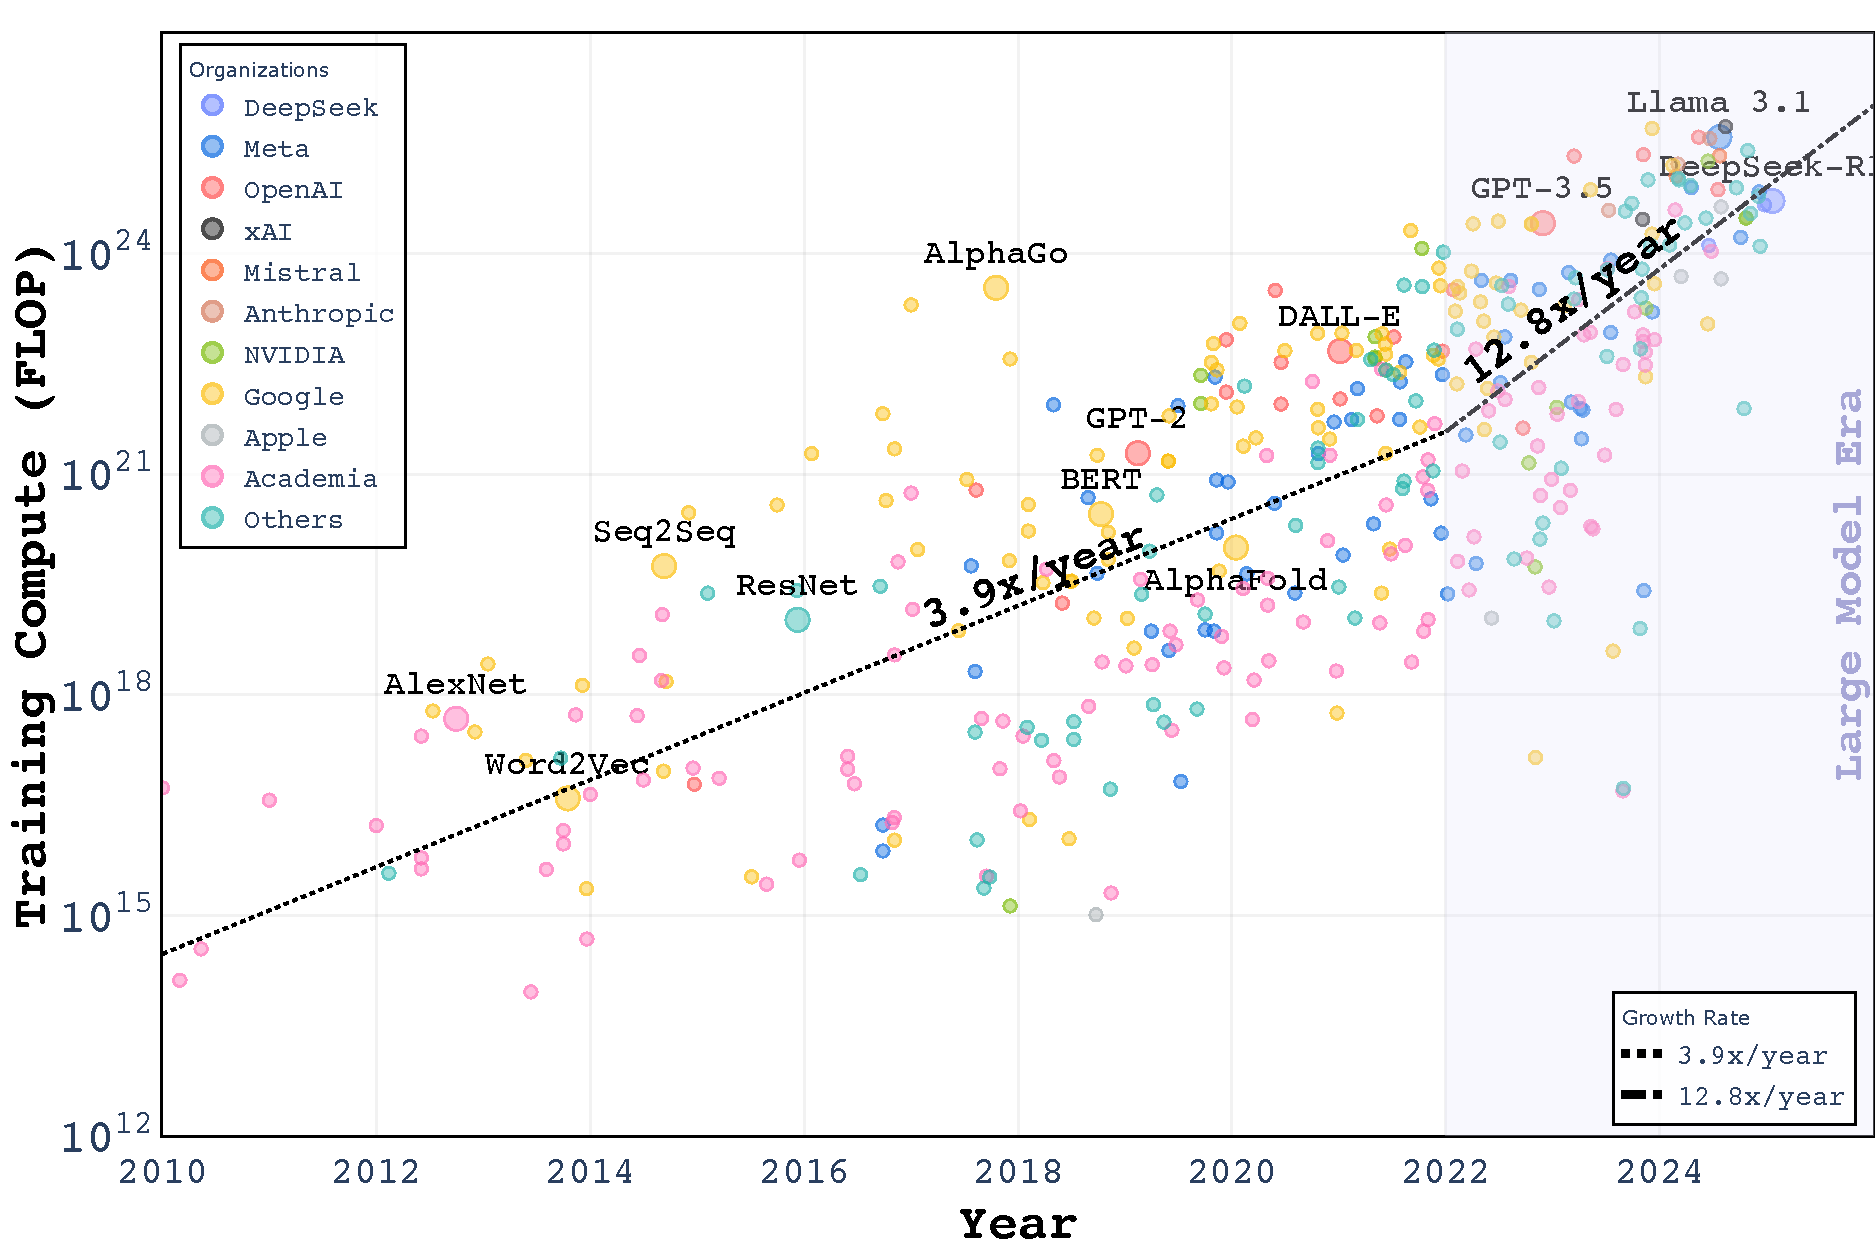
\includegraphics[width=\linewidth]{figs/ai_compute_trend.pdf}
    \vspace{-15pt} % Adjust vertical space if needed
    \caption{Trend of Computational Demand for Model Training. (Data source:~\cite{epoch2023trendsinmachinelearninghardware}).}
    \label{fig:model_comput_trend}
    \vspace{-12pt} % Adjust vertical space if needed
\end{wrapfigure}

\paragraph{Computational demand is growing exponentially.}
As large-scale AI models like GPT-4~\cite{openai2023gpt4}, Llama 3~\cite{meta2024llama3.1}, and DeepSeek-V3~\cite{liu2024deepseek} surpass the trillion-parameter scale, the global AI landscape faces severe computational efficiency challenges. As shown in Figure~\ref{fig:model_comput_trend}, since the deep learning revolution in 2010, AI training demands have grown at a super-exponential rate of 3.9$\times$ per year—an acceleration that intensified with the adoption of the transformer architecture as the industry standard \cite{vaswani2017attention}. With the advent of the era of large language models in 2022, the demand for computing power has surged even further, reaching an unprecedented growth rate of 12.8$\times$ per year. This marks a transformative shift in AI computation, where the need for computing power is expanding at an unprecedented pace, pushing the limits of existing hardware and infrastructure. \looseness-1




\paragraph{Moore's Law is slowing down.}
Moore's Law, which has driven the growth in computing power for decades, is slowing down as we approach the physical limits of silicon-based chip technology~\cite{kressel2023end}. The difficulty in shrinking transistors has led to diminishing returns in computational performance. As a result, the AI industry is relying more on specialized hardware like GPUs, TPUs, and custom chips to meet growing demands. However, this shift has made high-performance hardware even more expensive and exclusive, further intensifying the gap between organizations with the resources to develop advanced AI models and those without.

\paragraph{Infrastructure capacity is a constraint.}
The rapid expansion of AI model scales and the surge in computational demand are facing dual constraints in global computing infrastructure. On one hand, bottlenecks in advanced semiconductor manufacturing severely limit the expansion rate of AI data centers. The foundry capacity for wafers at 5nm and below—such as those produced by TSMC—has already been fully booked by leading technology companies until 2026~\cite{benzinga2024tsmc}. Moreover, the construction of new wafer fabs involves long lead times and is further constrained by the global supply chain shortages of critical equipment, such as lithography machines.
On the other hand, the exponential increase in chip deployment within individual AI clusters is putting immense pressure on the already limited semiconductor manufacturing capacity, pushing the industry toward its production ceiling~\cite{scaleflux2024ai}.
These factors have significantly hindered the continuous expansion of computing power, making it increasingly difficult to scale AI infrastructure sustainably.

\section{Scaling Beyond Limits: Opportunities from Edge Devices}
\label{sec:opportunities}

\subsection{Massive Data from Edges}
\label{subsec:edge_data}

As discussed in §~\ref{subsec:data_exhaustion}, edge data represents a crucial alternative to synthetic data in addressing the challenge of data exhaustion. Edge data refers to the data generated by edge devices at or near the source of data generation, which typically remains private and localized rather than being publicly accessible. Edge devices encompass a wide range of equipment including Internet of Things (IoTs) sensors, smartphones, wearables, industrial controllers, and other smart devices that process data at the network edge. 
Data generated at edges offers unique advantages in both data volume and data quality. \looseness-1


\begin{figure*}[htbp]
    \centering
    \begin{minipage}[t]{0.49\linewidth}
        \centering
        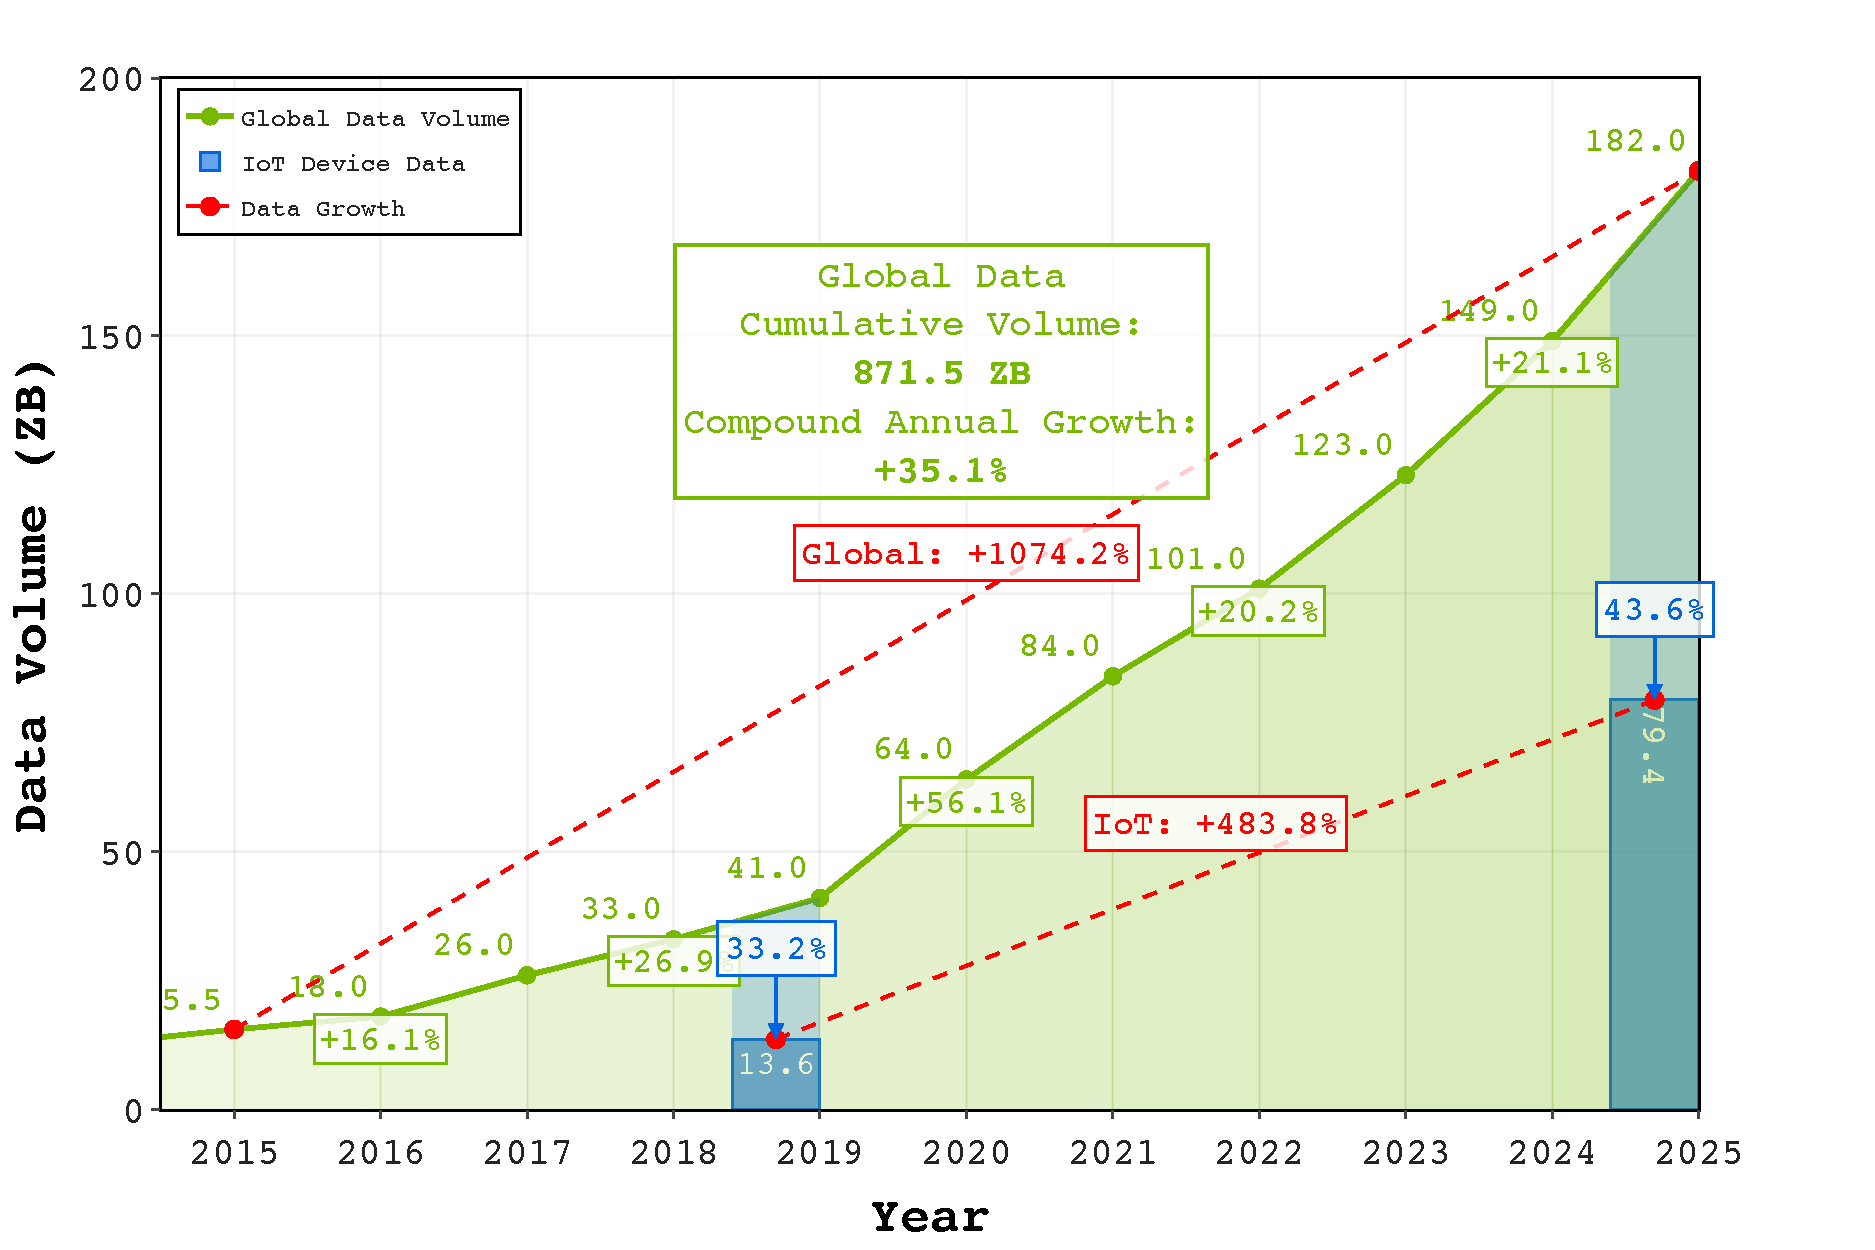
\includegraphics[width=\linewidth]{./figs/iot_data_contribution.pdf}
        % \vspace{-20pt}
        \caption{Global data volume from 2014 to 2025 and IoT device data volume in 2015 and 2025. (Data sources: Global data volume from \cite{statista_global_2023}; IoT device data volume from \cite{statista_iot_2023}.)}
    \label{fig:global_data}
    \end{minipage}
    \hfill
    \begin{minipage}[t]{0.49\linewidth}
        \centering
        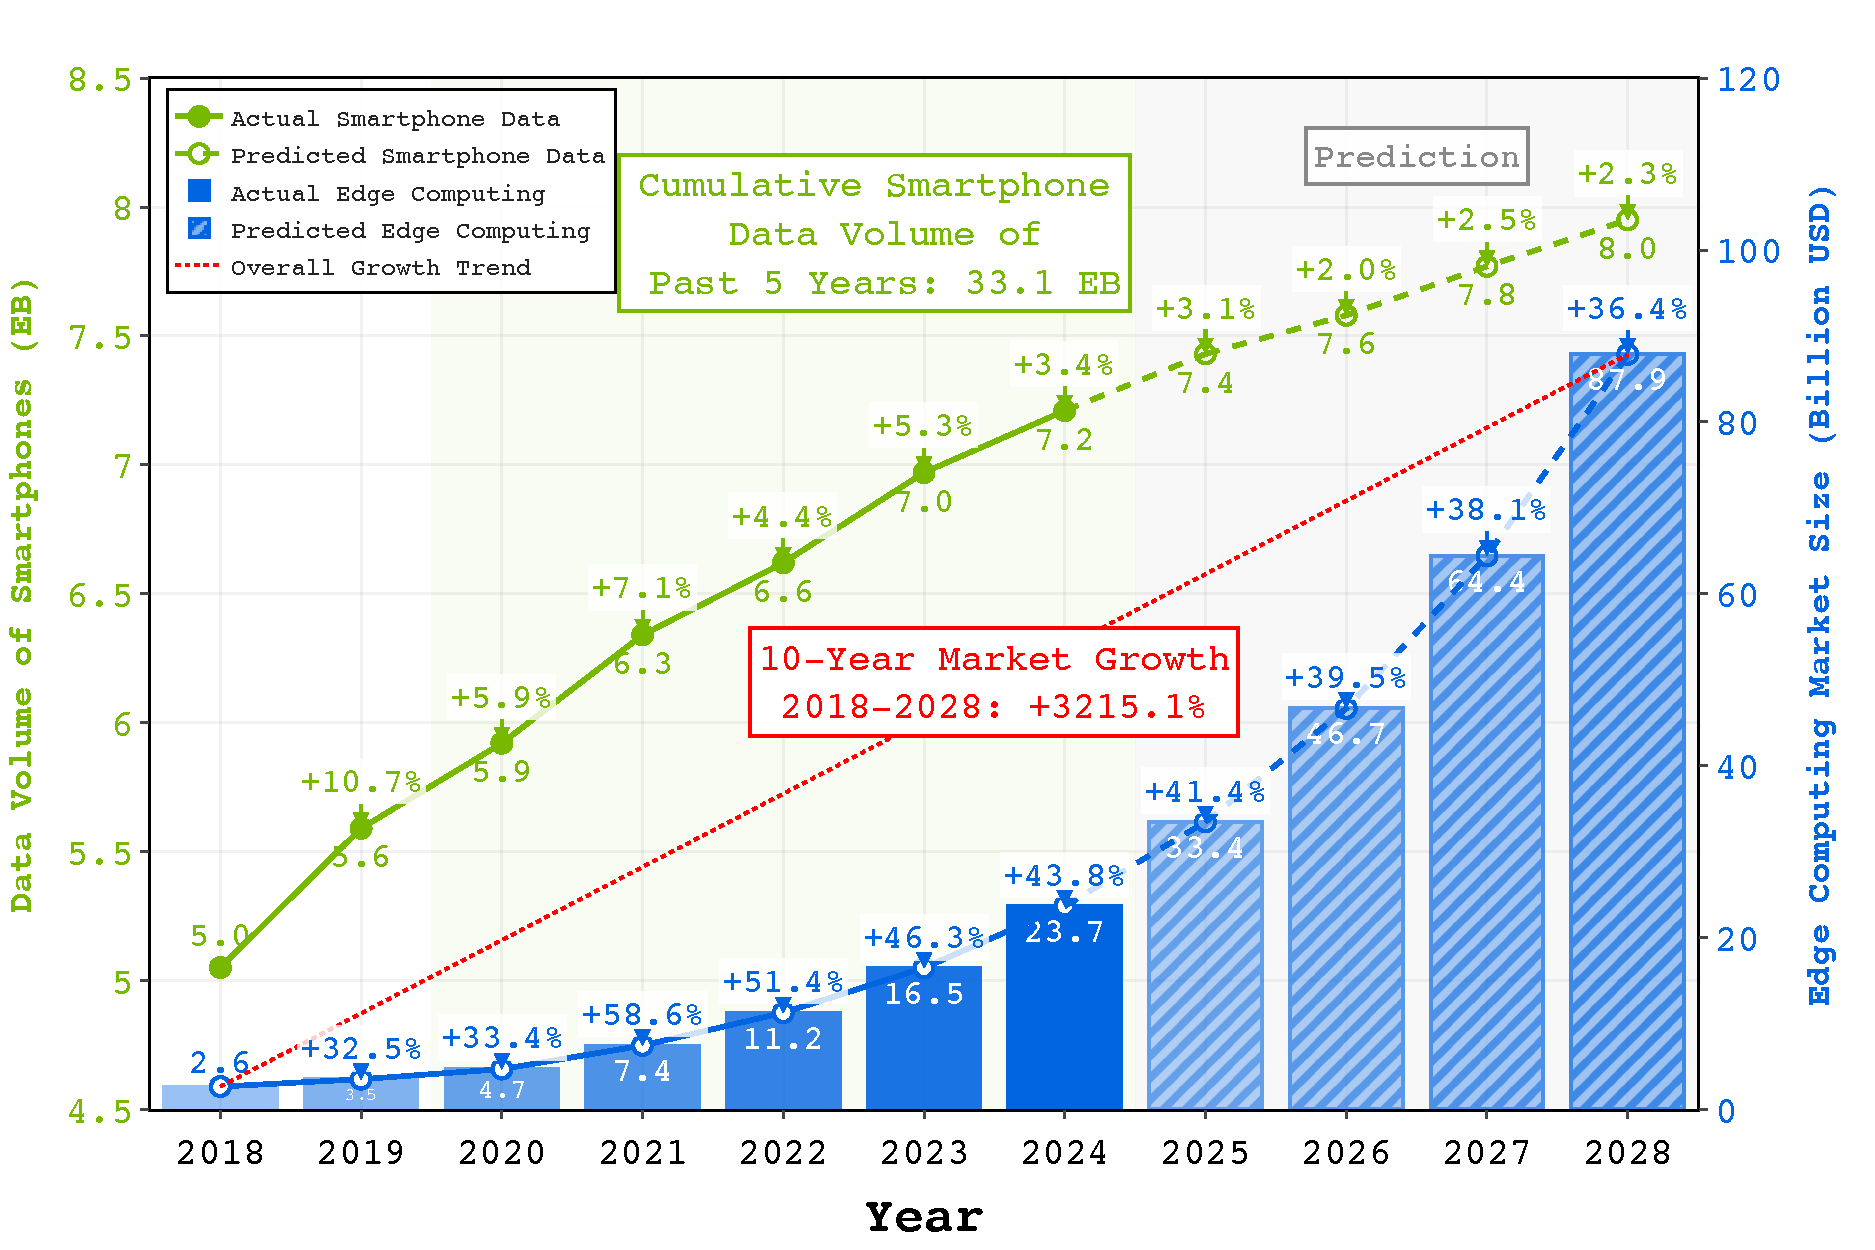
\includegraphics[width=\linewidth]{./figs/edge_and_smartphone.pdf}
        % \vspace{-20pt}

        \caption{Smartphone data volume with edge computing market size (right) from 2018 to 2028. (Data sources: Edge computing market \cite{grandview_edge_2023}; Smartphone data volume from \cite{bankmycell_smartphone_2023}.)}
    \label{fig:smartphone}
    \end{minipage}
    \vspace{-10pt}
\end{figure*}

\paragraph{Edge-generated data is explosively growing.} 
% By 2025, it is projected that over 80\% of global data will be generated directly at the edge, rather than in traditional centralized data centers \cite{seagate_rethinkdata_2020}. This shift highlights a fundamental transformation in how data is created, processed, and utilized across industries.
According to the statistical data from \cite{statista_global_2023,statista_iot_2023} (as illustrated in Figure~\ref{fig:global_data}), 
the global data volume is projected to reach 182 ZB by 2025~\cite{statista_global_2023}, where the data generated by IoT devices is anticipated to increase from 13.6 ZB in 2019 to 79.4 ZB in 2025~\cite{statista_iot_2023}, elevating its share of the global data volume from 33.2\% to 43.6\%, showing a particularly pronounced growth in edge-generated data. Over the period from 2015 to 2025, the global data volume exhibited a compound annual growth rate (CAGR) of 35.1\%, resulting in an overall increase of 1074.2\% and a cumulative total of 871.5 ZB. IoT device data experienced a growth of 483.8\% from 2019 to 2025. This trend underscores the increasingly central role of edge-generated data in the global data ecosystem.
Beyond IoT devices, smartphones, as a critical source of edge-side data, are also contributing to the steady rise in data volume. As depicted in Figure~\ref{fig:smartphone}, the estimated smartphone data volume is projected to grow from 5 EB in 2018 to 8 EB by 2028
\footnote{These numbers are estimated based on an average user data generation of 1 GB per device. For detailed estimation methodology, refer to Appendix \ref{app:smartphone_ethod}.}. 
This exponential growth is closely aligned with the rapid expansion of the edge computing market, which is forecasted to surge from \$5.5 billion in 2019 to \$87.9 billion by 2028, representing a remarkable growth rate of 3215.1\%. The burgeoning edge computing market has further catalyzed the generation and processing of edge-side data, reinforcing its significance in the broader data landscape 
\footnote{\cite{idc_seagate_dataage_2019,seagate_rethinkdata_2020} provide a more comprehensive overview of the global data volume, but we cannot access the statistics data. 
We appreciate any suggestions for better statistical data sources.
}.



\paragraph{Edge-generated data has distinctive advantages.} 
Beyond its impressive quantity, edge data possesses several distinctive characteristics that make it particularly valuable for model training.
First, edge data provides enhanced \textit{privacy} characteristics. Since edge data typically remains local to devices and does not need to be centrally stored, it allows for more privacy-preserving approaches to data utilization. This local-first nature enables compliance with increasingly strict data privacy regulations while still allowing the data to contribute to model training.
Second, edge data exhibits superior \textit{diversity} across multiple dimensions. It encompasses a wide variety of data types from IoT devices, mobile interactions, and personal devices, covering different domains, languages, and user behaviors. This natural diversity provides richer training signals compared to curated public datasets \cite{nayak2024review}. 
Third, edge data demonstrates strong \textit{real-time} capability. Unlike public datasets, which are often updated infrequently, edge devices continuously generate fresh data with low latency \cite{cavliwireless_edgecomputing}, offering more up-to-date and relevant training samples.
% Third, edge data offers enhanced \textit{personalization} characteristics. It enables real-time interactions and context-aware recommendations by leveraging local data such as location and device behavior. This allows for highly relevant and adaptive personalization that can dynamically adjust to user preferences \cite{xenonstack_edge_ai_2023}.
% Fourth, edge data exhibits enhanced \textit{context awareness} due to the proximal positioning of edge devices to data sources, enabling the capture of fine-grained contextual information often absent in public datasets. For instance, wearable devices collect synchronized activity and location data, providing high-fidelity behavioral patterns that preserve temporal and spatial context.
Despite these advantages, edge-generated data can present challenges such as low signal-to-noise ratios, unclean, or potentially harmful content. However, recent advancements in data quality assessment methods (e.g., data prospector \cite{ni2024small}), have emerged to identify and filter high-quality data from edge sources, ensuring that only the most reliable and valuable data is selected for model training.

In conclusion, edge data with its explosive growth and distinctive characteristics, is a valuable resource for model pretraining. Its diversity, real-time nature, personalization, and rich context make it an ideal foundation for developing robust and adaptable large-scale models, enhancing their ability to serve real-world applications effectively.

% \vspace{-0.5cm}
\begin{insights}
    \textbf{Insight:} The smartphone data volume of the past 5 years (before 2025) is projected to reach approximately 33.1 EB, with unique advantages in privacy, diversity, and real-time context, demonstrating the massive data potential of edge for AI model training.
\end{insights}
   



\subsection{Massive Computing Power from Edges}\label{subsec:edge_compute}



\paragraph{Edge computing power is growing rapidly.}
In recent years, edge computing has experienced explosive growth in computing power, driving smart devices to evolve from single-function tools into multimodal perception and decision-making centers. For instance, as shown in Figure~\ref{fig:edge_trend}, flagship smartphones such as the iPhone 16 series, equipped with 3nm process chips, have achieved computing power exceeding 2 TFLOPS~\cite{apple2024iphone16pro}, enabling local execution of complex AI tasks like real-time image enhancement and multilingual speech translation. 
Notably, the computing power of an individual smartphone has potentially surpassed that of laptops in the same period.
The breakthroughs are even more pronounced in the desktop sector,
% where NVIDIA's GeForce RTX 5090, with 104.9 TFLOPS of computing power~\cite{nvidia2025}, 
achieving an annual computing power growth rate of 1.29$\times$/year, surpassing that of smartphones and laptops (both 1.20$\times$/year). 
% \footnote{{Data source: \url{https://nanoreview.net}.}}
These three types of devices form a differentiated growth hierarchy, collectively driving edge computing's overall computing power to expand at an annual average rate of 1.28$\times$/year.
% , significantly outpacing the 1.3$\times$ growth rate of cloud computing~\cite{epoch2023trendsinmachinelearninghardware}, with the gap between the two continuing to narrow. 
This growth is fueled by three key technological drivers: advanced manufacturing processes (3nm technology increases transistor density by 60\%~\cite{apple2024iphone16pro}), dedicated architectures (modern smartphone SoCs integrate NPUs for AI acceleration), and scenario-driven innovation (e.g., autonomous driving demands end-to-end latency of less than 100ms~\cite{nvidia2023}).
% The quantitative increase in computational power has led to qualitative transformations: AR/VR devices can now reduce spatial modeling latency from seconds to milliseconds~\cite{idtechex2024}; medical-grade wearable devices can perform real-time analysis of 12-lead ECG data~\cite{gopala2022edge}; and educational tablets are capable of rendering 8K-resolution holographic teaching environments~\cite{precedence2024}. 
% These advancements have elevated edge computing from a supporting role to a core enabler of intelligence. The rapid growth of the global edge AI chip market~\cite{cognitive2024} further underscores the trend of computing power shifting toward the edge. 

\begin{figure*}[htbp]
    \centering
    \begin{minipage}[t]{0.49\linewidth}
        \centering
        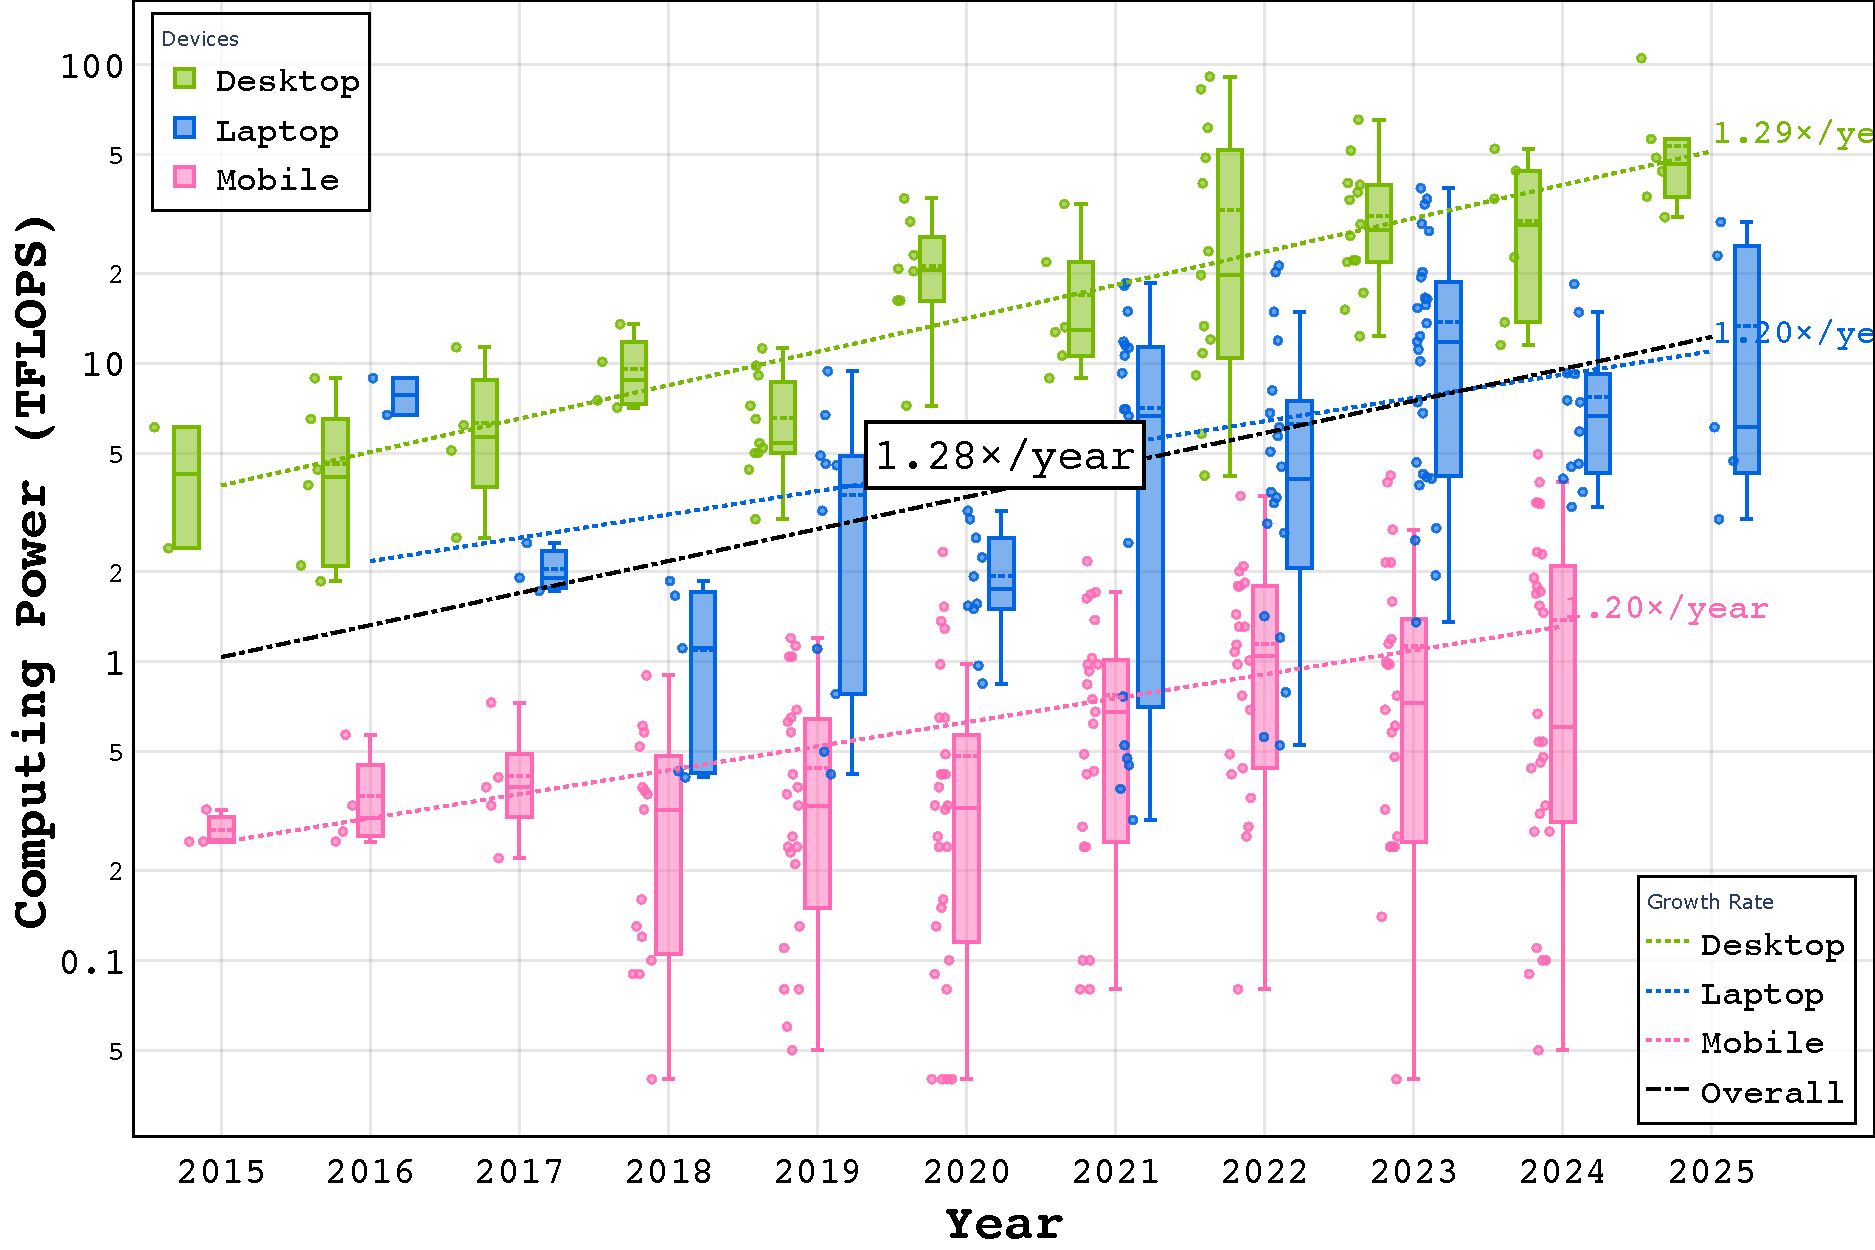
\includegraphics[width=\linewidth]{./figs/edge_compute_trend.pdf}
        % \vspace{-20pt}
        \caption{Edge Computing Power Evolution Trend. (Data source: \cite{nanoreview2025}).}
        \label{fig:edge_trend}
    \end{minipage}
    \hfill
    \begin{minipage}[t]{0.49\linewidth}
        \centering
        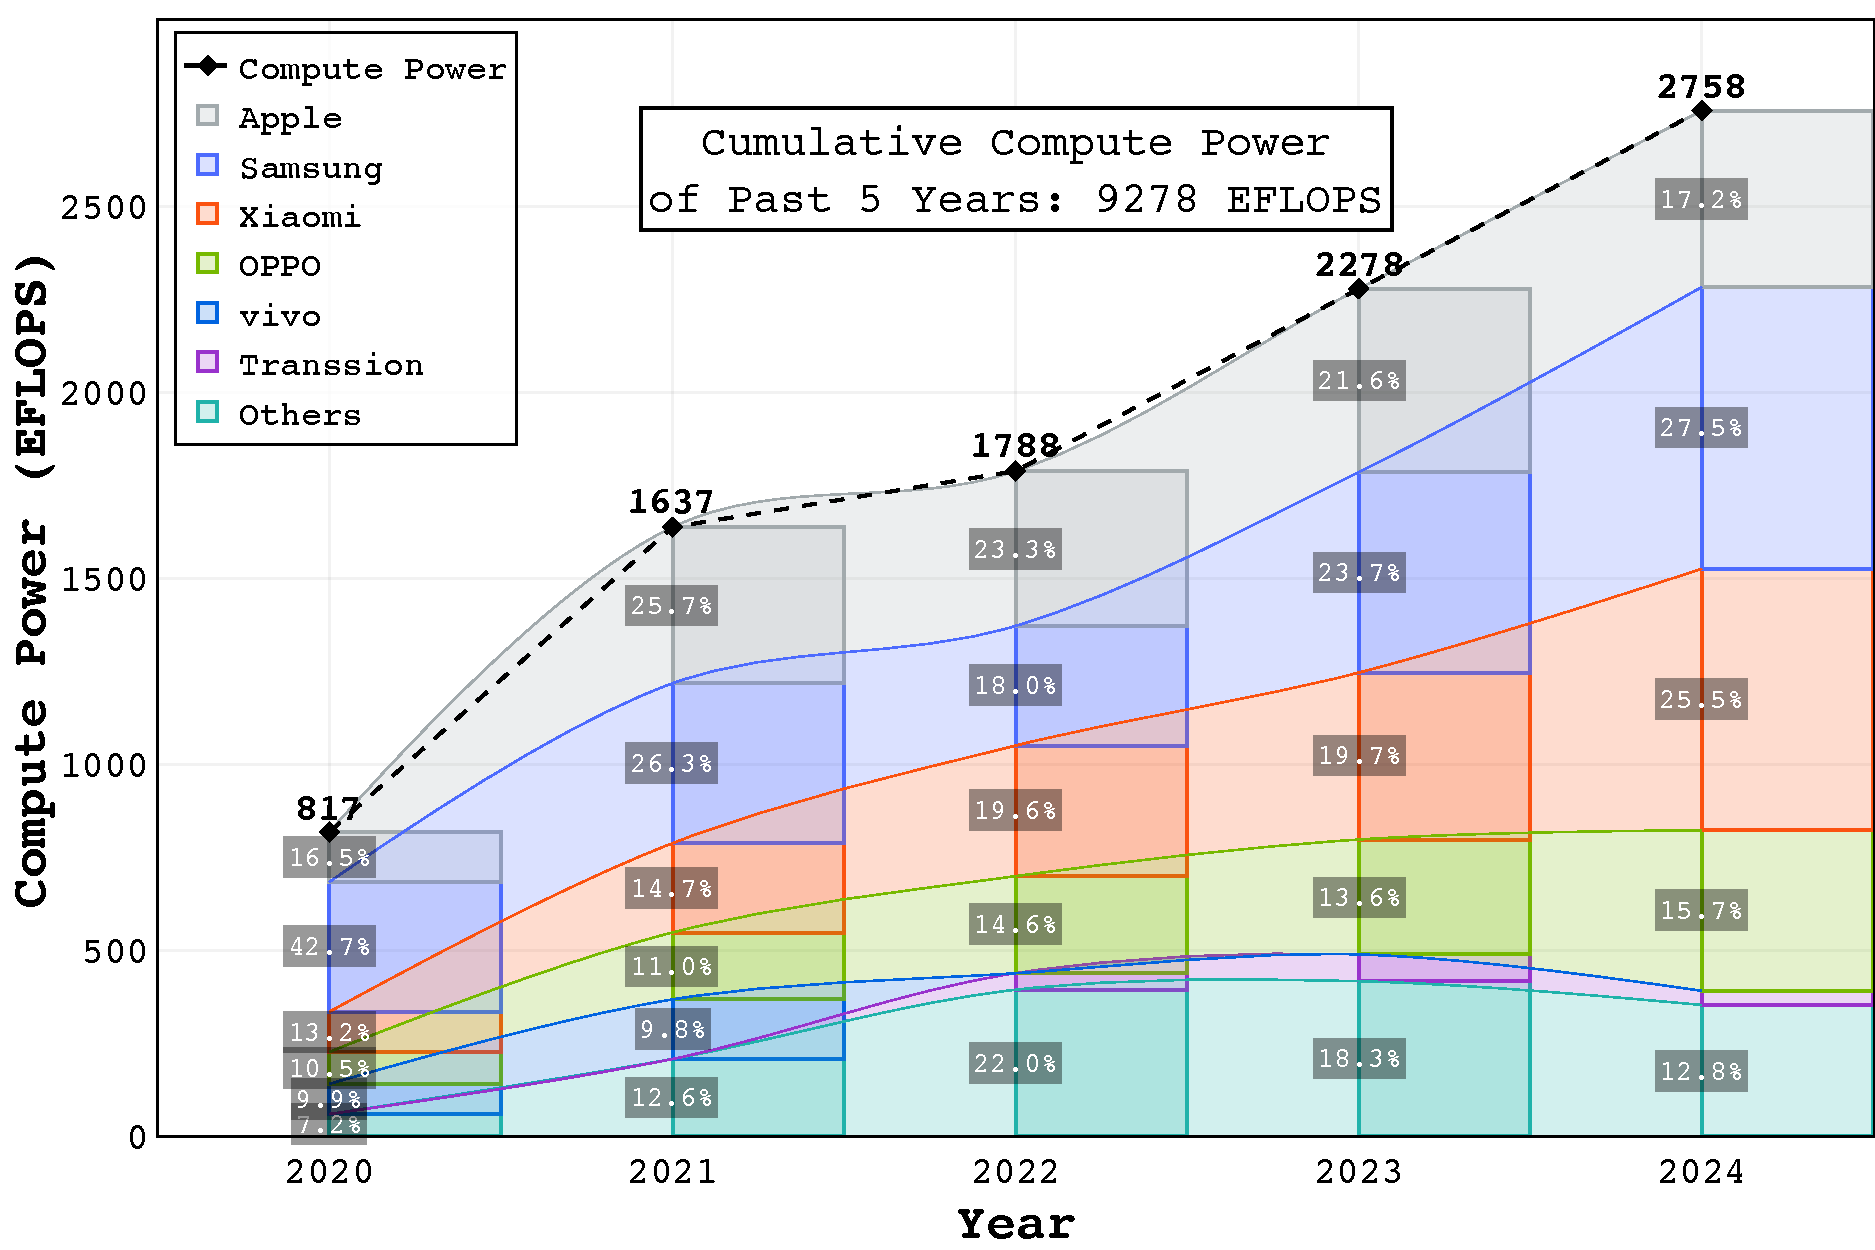
\includegraphics[width=\linewidth]{./figs/smartphone_compute_trend.pdf}
        % \vspace{-20pt}
        \caption{Smartphone Market Share and Computing Power Trends. (Data source: \cite{canalys2025}).}
        \label{fig:smartphone_trend}
    \end{minipage}
    \vspace{-10pt}
\end{figure*}


\paragraph{Edge computing has potential for LLM training.}
We analyze the performance of smartphone chips, representing typical edge devices, and estimated their overall computing power.
% , as summarized in Table~\ref{tab:chip_performance}. 
To ensure our estimation is as accurate as possible, we based our calculations on the market share data from \cite{canalys2025}.
We then estimated the total computing power of newly produced mobile devices by averaging the chip performance of each brand.
From 2020 to 2024, smartphone chip performance has seen significant improvements, with peak computing power increasing from 1.53 TFLOPS to 4.95 TFLOPS, and average computing power rising from 0.48 TFLOPS to 1.38 TFLOPS. Meanwhile, the overall computing power of mobile devices has grown from 817 EFLOPS in 2020 to 2,758 EFLOPS in 2024, and totally 9278 EFLOPS for past 5 years. This trend highlights the rapid expansion of edge computing power, which is not only essential for AI applications but also holds the potential for training complex AI models.
For instance, training the DeepSeek-v3~\cite{liu2024deepseek} model utilizes 2048 H100 GPUs, each providing a peak FP32 performance of 59.30 TFLOPS, resulting in a total computational capacity of 121,446.4 TFLOPS. If this workload were distributed across edge devices with a peak performance of 2 TFLOPS (e.g., mobile chips like the iPhone 16 series), approximately 60,723 users with edge devices working (\textit{ideally}) in parallel would be required to match the computational capacity. \looseness-1

\begin{insights}
    \textbf{Insight:} 
    The smartphone computing power of the past 5 years (before 2025) is projected to reach approximately 9278 EFLOPS, with individual flagship devices now achieving over 2 TFLOPS performance. The combined parallel computing power of approximately 30 iPhone devices (with A18 chips) can match the computational capacity of a professional AI training GPU (H100 with 59.30 TFLOPS). 
\end{insights}

However, current smartphone chips are primarily optimized only for inference efficiency rather than training capabilities. 
\textit{We advocate for and predict a future trajectory of edge computing where smartphone chip designs will increasingly prioritize and optimize on-device model training capabilities.
% , fundamentally transforming the edge computing landscape.
}
As computational power grows and distributed algorithms develop, we expect a paradigm shift enabling collaborative model training across networks of edge devices. This evolution positions the edge computing ecosystem as a critical catalyst for democratizing AI development and driving the next wave of innovations in the field.




\section{Technical Advancements}\label{sec:technical_advancements}

\subsection{Small Language Models at Edges}\label{subsec:small_language_models}


The first move of AI to Edge is to deploy small language models (SLMs) to edge devices \cite{lu2024small,wang2024comprehensive,van2024survey}. This trend is driven by the growing demand for AI applications that can run directly on edge devices, motivated by needs for privacy, offline usage, and real-time processing without cloud dependence. However, edge devices have limited memory, computation, and energy resources, requiring more efficient and compact models.


\paragraph{SLMs leverage innovative architectures for efficient edge deployment.}
The classic Transformer architecture \cite{vaswani2017attention} uses self-attention mechanisms for effective sequence modeling but faces quadratic complexity challenges, with models like TinyBERT \cite{jiao2020tinybert} (14.5M parameters) and ALBERT \cite{lan2020albert} (12M parameters) demonstrating its effectiveness at small scales. Mamba \cite{gu2023mamba}, based on state space models, achieves linear complexity and faster inference by utilizing only the previous hidden state, as demonstrated by Zamba2-2.7B \cite{glorioso2024zamba2} which achieves twice the speed and 27\% reduced memory overhead compared to traditional models. Hymba \cite{dong2024hymba} combines both approaches by integrating attention and SSM heads within the same layer for parallel processing, with its 1.5B variant trained on DCLM-Baseline-1.0 and SmolLM-Corpus achieving 11.67 times cache size reduction while outperforming Llama-3.2-3B. The xLSTM architecture \cite{beck2024xlstm} modernizes LSTM with exponential gates and matrix memory cells, with models ranging from 125M to 1.3B parameters trained on 300 billion tokens from SlimPajama \cite{cerebras2023slimpajama}, consistently outperforming comparable RWKV-4 \cite{peng-etal-2023-rwkv}, Llama \cite{touvron2023llama3}, and Mamba models across various tasks in the PALOMA benchmark \cite{magnusson2024paloma}. These architectural innovations demonstrate the potential for efficient and powerful language models that can run effectively on edge devices.


\paragraph{SLMs can be constructed through diverse methodological approaches.}
The construction of efficient SLMs relies on a comprehensive suite of techniques, each with specific performance trade-offs. 
For training SLMs from scratch, optimized MLM approaches \cite{devlin2019bert} with increased masking ratio (25\% vs traditional 15\%) demonstrate 2-3\% performance improvements for models under 3B parameters.
When deriving SLMs from existing LLMs, knowledge distillation has proven particularly effective, with response-based distillation \cite{sanh2019distilbert} reducing model size by 40\% while maintaining 95\% of the original performance.
In architecture optimization, the Mixture of Experts approach \cite{fedus2022switch} enables 65\% parameter reduction while potentially improving performance in specific tasks. Domain specialization has shown remarkable results, particularly in the medical field where 3B parameter models achieve 92\% accuracy, outperforming 175B models (89\%) \cite{fu2023specializing}.
The combination of these techniques yields impressive results - a notable example is a 770M parameter model from \cite{hsieh2023distilling} that combines distillation, quantization, and domain specialization to achieve 95\% of the performance of a 540B model on specific tasks while requiring less than 0.15\% of the computational resources. Most successful SLMs achieve their efficiency by combining multiple techniques, typically starting with knowledge distillation, applying compression methods, and finishing with domain-specific fine-tuning. 
\cite{wang2024comprehensive} has provided a comprehensive survey of SLMs, and we summarize the architecture innovations and training methods in Appendix \ref{app:slm_architectures_training}. \looseness-1


Despite remarkable progress in deploying compressed models to edge devices, the current landscape remains largely confined to individual devices operating in isolation, failing to leverage the massive distributed computing power that could be achieved through collaborative training across edge devices. This represents a significant missed opportunity, as the collective computing resources of billions of edge devices worldwide remain untapped, while individual devices struggle with the computational demands of modern AI applications.

\subsection{Collaborative Inference at Edges}\label{subsec:collaborative_inference}
The emergence of collaborative inference at the edge represents a significant shift in AI infrastructure, enabling more accessible and cost-effective AI solutions compared to traditional data centers which often present barriers in terms of cost, energy consumption, and accessibility. Recent frameworks like Exo \cite{exo} enable users to create AI clusters using everyday devices such as phones, tablets, and computers through peer-to-peer architecture, effectively unifying their computational resources.

Several approaches advance this paradigm: Neurosurgeon \cite{kang2017neurosurgeon} introduces a lightweight scheduler that partitions DNN computations between devices and datacenters; MoE$^2$ \cite{jin2025moe2} optimizes LLM inference under energy and latency constraints; Edgent \cite{li2018edgent} enables low-latency edge intelligence through adaptive partitioning and early-exit mechanisms; and Galaxy \cite{ye2024galaxy} leverages hybrid model parallelism to efficiently execute Transformer models across edge devices. Despite these advances, the current landscape has yet to fully capitalize on the potential of distributed data resources at the edge. The next frontier lies in transforming these devices from mere inference endpoints into active training participants, representing a significant opportunity for distributed AI development. \looseness-1

\subsection{Feasibility of On-Device Training}

Recent advancements in optimization techniques have significantly reduced the memory and computational requirements for training machine learning models, making on-device training increasingly feasible, even on resource-constrained edge devices.
For instance, Lin et al. \cite{lin2022ondevice} demonstrated training neural networks on microcontroller units with only 256KB of RAM by employing an algorithm-system co-design framework. 
% Their approach includes Quantization-Aware Scaling to stabilize 8-bit quantized training and Sparse Update to skip gradient computation of less important layers, making it particularly suitable for resource-constrained environments.
Similarly, Cai et al. \cite{cai2020tinytl} introduced a tiny transfer learning approach that freezes most parameters and only trains a small subset, allowing effective fine-tuning with minimal memory requirements. Qiu et al. \cite{qiu2022zerofl} proposed ZeroFL, a framework that relies on highly sparse operations to accelerate on-device training in federated learning settings, enabling efficient model training on edge devices with up to 95\% sparsity.
Recent work by Sugiura and Matsutani \cite{sugiura2025elasticzo} further advanced this field with ElasticZO, which combines zeroth-order and first-order optimization to achieve a better trade-off between accuracy and training cost. Their ElasticZO-INT8 variant achieves integer arithmetic-only training, further reducing memory usage and training time by approximately 1.5x without compromising accuracy.
% Zeroth-order methods have also been extended to federated learning for large language models as demonstrated by Ling et al. \cite{ling2024convergence}, who showed that memory-efficient zeroth-order optimization can reduce GPU memory usage during training to levels comparable to those during inference.
These advancements suggest that on-device training is no longer limited to high-end devices with abundant resources. Even small embedded systems with memory capacities measured in kilobytes rather than gigabytes can participate in model training.\looseness-1

\subsection{Collaborative Training at Edges}\label{subsec:collaborative_training}

To harness the potential of vast amounts of data distributed across numerous devices, we envision a future where everyone can participate in training large-scale models. Federated learning emerges as a paradigm for distributed collaborative training that makes this vision possible.


\textbf{Federated learning} \cite{mcmahan2017communication} is a practical paradigm that enables collaborative model training while preserving data privacy. Instead of collecting raw data from edge devices, which may violate privacy regulations like GDPR \cite{regulation2018general}, this approach distributes the training process across multiple devices. Each device trains on its local data and only shares model updates with the central server. This approach can effectively utilizes both computational and data resources available at edges.


\textbf{Federated LLMs for fine-tuning}
has emerged as a critical direction in recent research of large language models, addressing the challenges of privacy preservation and resource constraints. FlexLoRA \cite{bai2024federated} introduces a novel framework that enables efficient fine-tuning of large language models in a federated setting, demonstrating comparable performance to centralized fine-tuning while maintaining data privacy. FedFM \cite{yang2025federated} tackles the critical challenges of system and statistical heterogeneity in federated learning, proposing adaptive optimization techniques that improve model convergence across diverse client devices.
To address the computational constraints of edge devices, FedPETuning \cite{zhang2023fedpetuning} employs parameter-efficient fine-tuning techniques, significantly reducing the memory and computation requirements while maintaining model performance. This approach enables even resource-constrained devices to participate in the fine-tuning process. Similarly, \cite{chen2024feddat} bridges the gap between federated learning and foundation models by introducing novel techniques for efficient knowledge transfer and model adaptation in multi-modal heterogeneous federated learning settings.
In domain-specific applications, FedMatch \cite{chen2021fedmatch} demonstrates the effectiveness of federated learning for question-answering tasks, showing that models can be fine-tuned on sensitive domain-specific data while preserving privacy. These advancements are supported by open-source frameworks like Flower \cite{Flower} and FATE-LLM \cite{fan2023fate}, which provide robust platforms for implementing federated fine-tuning of large language models. 



\textbf{Federated LLMs for pretraining} 
have opened up exciting new possibilities for large language model training. Rather than relying on traditional data center approaches, researchers have developed innovative geographically distributed frameworks that enable collaborative training across many devices.
% This shift represents a fundamental change in how we think about training large models, moving away from centralized computation towards more distributed, privacy-preserving architectures that can potentially leverage the computational resources of millions of edge devices.
% Recent advancements in decentralized and federated learning frameworks have made significant strides in the training of large-scale models. 
Notably, Prime Intellect \cite{OpenDiLoCo} has launched the first decentralized training project for a 10 billion parameter model, named INTELLECT-1, which utilizes the OpenDiLoCo framework to significantly reduce communication costs between nodes. This innovative approach allows for dynamic management of computational resources across multiple locations, achieving an impressive 83\% overall computational utilization while collaborating with up to 112 H100 GPUs across five countries and three continents. The model not only enhances parameter efficiency by 25 times but also demonstrates robust performance in various benchmark tests.
In parallel, the Flower Lab \cite{Flower} has introduced FlowerLLM, which successfully trained a 1.3 billion parameter large language model (LLM) using novel federated learning methods. 
Additionally, it has also developed Photon \cite{sani2024photon}, an open-source framework that provides flexible configurations for training models of different sizes, making federated LLM training more accessible to a broader range of participants and computational resources. \looseness-1

These frameworks underscore a shift towards decentralized AI inference and training (summarized in Appendix~\ref{app:distributed_collaborative_frameworks}), enabling researchers worldwide to contribute to advanced model development without the constraints of centralized resource control, thus paving the way for a more collaborative and inclusive AI landscape. \looseness-1



\section{An Open Problem: How to Train LLMs with Small Edge Devices?}\label{sec:open_problem}


A fundamental limitation of traditional federated learning lies in its requirement for each participant to maintain and train a complete model locally. This assumption becomes particularly problematic in the context of large language models, where the computational and memory requirements far exceed the capabilities of most individual participants. For instance, in sensitive domains like healthcare~\cite{bolton2024biomedlm}, multiple hospitals may wish to collaboratively train a medical language model to leverage their collective data while maintaining data privacy. However, traditional federated learning mandates that each participating hospital possess sufficient computational resources to train the complete model locally. Despite these institutions' valuable data contributions and their motivation to enhance model capabilities through collaborative training, many hospitals lack the necessary infrastructure to participate effectively. This resource constraint significantly limits the potential for collaborative model training in critical domains where data privacy is paramount but computational resources are unevenly distributed \cite{kairouz2021advances}. 
\begin{figure}
    \centering
    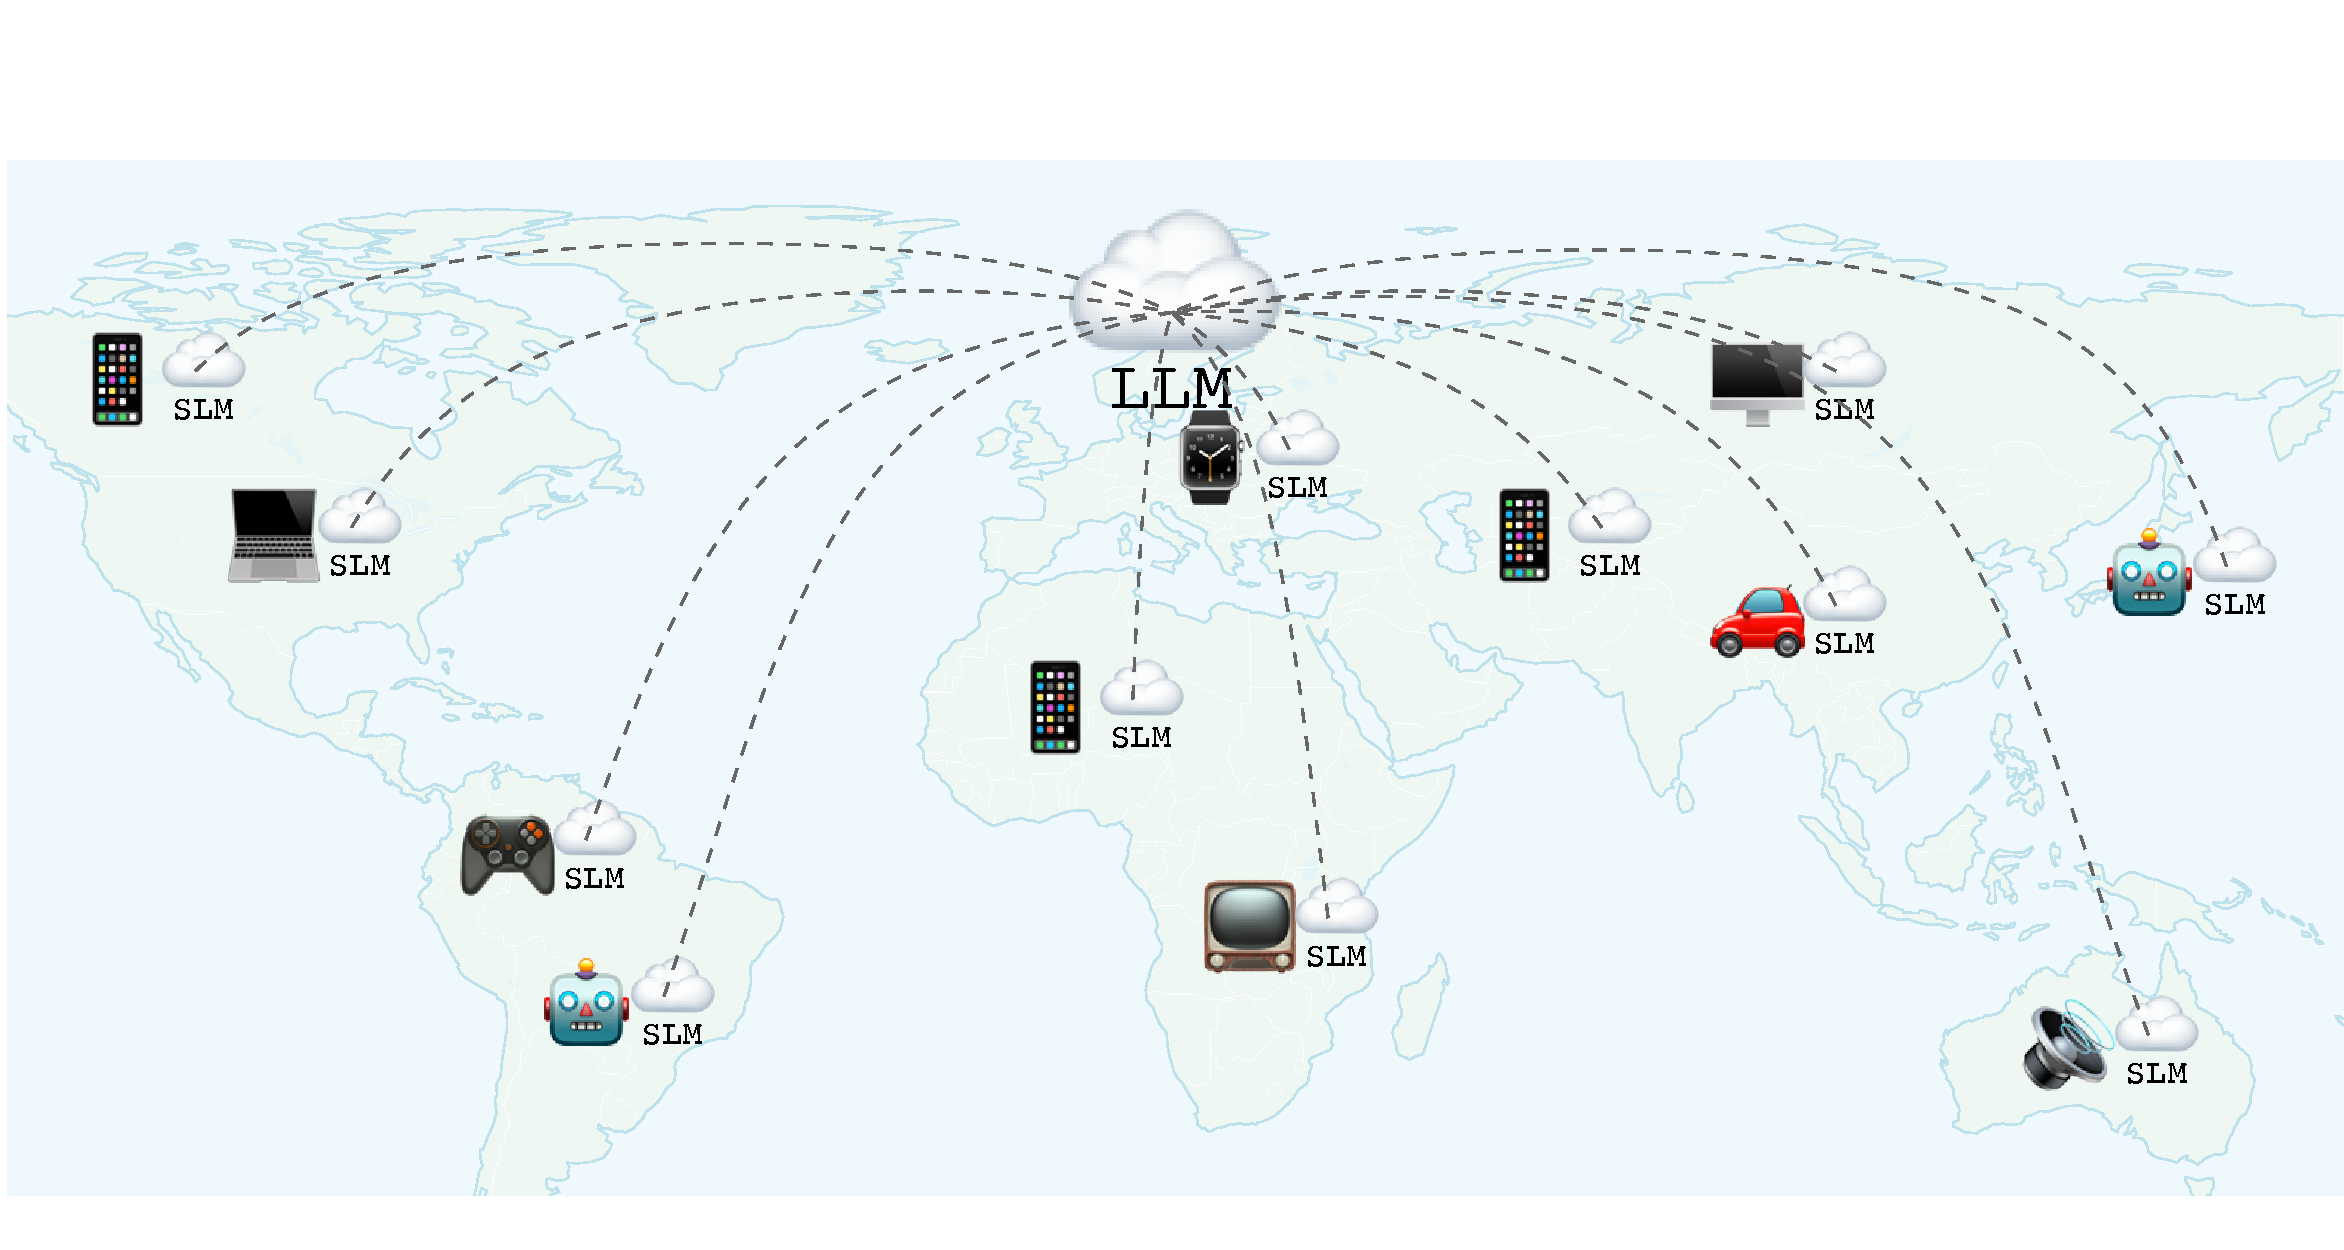
\includegraphics[width=0.8\linewidth]{./figs/fedllm.pdf}
    % \vspace{-20pt}
    \caption{Train Large Language Models with Small Edge Devices}
    \vspace{-15pt}
    \label{fig:fedllm}
\end{figure}
While some federated learning approaches allow training partial model parameters \cite{horvath2021fjord,alam2022fedrolex}, the enormous disparity between large language models and what edge devices can train—often orders of magnitude smaller due to inherently constrained resources—remains too vast to be effectively bridged by current FL frameworks.
Therefore, we need to develop a new federated learning paradigm that enables participants to collaboratively train a large language model even under extremely limited resources (as shown in Figure~\ref{fig:fedllm}).
\textbf{It is still an open problem to train large language models with small edge devices.} Therefore, we encourage the research community to develop novel distributed collaborative computing methods in two key directions:

\subsection{Heterogeneous Device Model Fusion: from Small to Large}\label{subsec:model_fusion}

The first direction addresses the fundamental challenge of model size disparity in federated learning. Modern large language models typically contain hundreds of billions of parameters, while edge devices have severely limited computational resources. This creates an enormous scale gap - the large target model may be hundreds or even thousands of times larger than what individual devices can handle. To bridge this gap, each edge device should run a small language model that matches its computational capacity. For example, while the central model may have 100 billion parameters, a resource-constrained mobile device might only handle a 100-million parameter model, representing a 1000x size difference. 
The key challenge then becomes how to effectively aggregate and fuse knowledge from these much smaller models into the large target model. 
We need novel techniques that can meaningfully combine insights from models operating at radically different scales while preserving the unique contributions of each small model. This requires fundamentally rethinking traditional model fusion approaches \citep{velasevic2023effects,azizan2019distributed} to handle such extreme parameter count disparities.

\subsection{Heterogeneous Device Compute Sharing: from Node to Cluster}\label{subsec:compute_sharing}

The second direction is to enable efficient compute resource sharing across heterogeneous devices by treating them as a unified compute cluster rather than independent nodes. Consider a smart home environment where multiple devices—smartphones, laptops, and desktop computers—could form a collaborative compute cluster. While each individual device has limited resources, their collective computing power could be substantial. For example, a laptop could handle intensive computational tasks, smartphones could manage coordination and lightweight processing, and desktop computers could contribute their onboard computing power. Meanwhile, other IoT devices such as smart speakers, security cameras, and vehicles could serve as data sources, providing valuable real-world inputs like voice commands, visual feeds, and environmental parameters. The language model would effectively run and train across this entire device cluster, leveraging both computing power and diverse training data from the environment.
This distributed execution requires new frameworks that can intelligently decompose and distribute model computations based on each device's capabilities and current load. The system must dynamically balance workloads - when the security cameras are idle at night, they could take on additional compute tasks, while during peak usage hours, the load could shift to other devices. 
This requires innovations in real-time resource allocation, task scheduling across heterogeneous hardware, and efficient inter-device communication protocols to ensure the collective computing power is optimally utilized \citep{zhao2024retrieval}.

% \section{Alternative Views}
% \paragraph{Challenges of edge-generated data}
While edge devices collectively offer tremendous potential with massive amounts of data and computational resources, effectively utilizing this potential remains a significant challenge. 
The fundamental challenge in leveraging edge data for large model pre-training lies in its inherent \textit{data heterogeneity} and \textit{system heterogeneity}. 
Data heterogeneity encompasses varying quality standards, formats, and local statistical distributions, while system heterogeneity involves diverse computational capabilities, memory constraints, and resource availability,which has been a core challenge in federated learning \cite{mcmahan2017communication}. 
Furthermore, decomposing large model training tasks across multiple resource-constrained edge devices and efficiently aggregating their results to a large one remains an extremely challenging problem.
This area will continue to attract increasing research attention in the future to make the dream come true.
% Fortunately, large language models possess a unique advantage in this context - their significant model capacity and sophisticated architectures allow them to effectively capture and model diverse data distributions simultaneously, making them particularly well-suited for learning from heterogeneous edge data sources.


% \paragraph{Challenges of edge computational resources} The fundamental challenge in leveraging edge computing for large model training lies in its inherent \textit{computational heterogeneity}. While edge devices collectively provide massive computing power compared to centralized training, effectively coordinating and utilizing this distributed computing power remains a significant technical challenge \cite{kairouz2021advances}.
% The heterogeneity manifests in varying computational capabilities, memory constraints, and distinct resource availability patterns that reflect different device types and usage scenarios. 
% To address these challenges, novel distributed training architectures and optimization techniques need to be developed that can effectively handle device heterogeneity while ensuring training efficiency and model quality. This includes adaptive resource allocation strategies, asynchronous training methods, and robust fault tolerance mechanisms.




\section{Conclusion}

In this position paper, we have argued that 
leveraging massive distributed edge devices can break barriers of data and computing wall, and everyone can participate in training large models with small edge devices.
Our comprehensive analysis demonstrated the vast untapped potential of edge resources, with smartphone data volume reaching approximately 33.1 EB and a combined computing power of around 9278 EFLOPS  in the past 5 years. 
These edge resources offer unique advantages in terms of data diversity, privacy, real-time context, and computing efficiency. 
% While significant challenges remain in managing heterogeneity and coordination across distributed systems, 
This paradigm shift towards distributed training could democratize AI development and open an exciting new chapter in the scaling of foundation models.



\bibliography{st,zdd,zzy}
\bibliographystyle{iclr2026_conference}

\newpage
\appendix
\section{Impact Statements}\label{sec:impacts}

The shift from centralized to distributed training of large models, may introduce new technical and societal challenges and have the potential to fundamentally reshape the AI landscape. 


\subsection{AI Monopoly and Democratization}\label{subsec:ai_monopoly_and_democratization}


The current AI landscape is characterized by significant concentration of power among a few tech giants, primarily due to their monopoly over massive computing resources and data centers \cite{bommasani2021opportunities}. This monopolistic trend has intensified with companies like OpenAI increasingly moving towards closed systems. 
While open-source alternatives like Llama \cite{touvron2023llama3}, Deepseek \cite{liu2024deepseek} and other community-driven models have made strides towards democratization by releasing model parameters and technical reports \cite{welsh2024democratising}, the gap in computational resources and data access between major AI companies and other players remains substantial and continues to widen. 
This disparity in resources allows tech giants to maintain their absolute dominance in determining the direction of AI development, raising concerns about AI democratization. 


Edge device-based collaborative training presents a promising pathway to democratize AI development \cite{yao2022edge}.
By leveraging the collective computing power of millions of edge devices, this approach could effectively challenge the existing monopolistic structure \cite{dong2025beyond}. 
This democratization of AI training through edge devices could fundamentally reshape the structure of responsibilities and authorities.
If everyone can participate in training LLMs, the AI landscape could fundamentally change. Training decisions would shift from companies to communities, creating shared responsibility for model development \cite{zeng2023distributed}. Global participation would help models reflect diverse cultural perspectives, while allowing communities to adapt models for their local needs.
Furthermore, this decentralized approach could foster a more competitive and innovative AI ecosystem. When the barriers to entry for AI model training are lowered, we can expect to see a broader range of specialized models emerging (like \cite{song2025injecting,MedicalGPT,li2023large,yao2024lawyer,AlphaEvolve}), better suited to local needs and diverse use cases.


\subsection{Fairness and Incentive Mechanisms}\label{subsec:fairness_and_incentive_mechanisms}

The distributed training paradigm introduces new considerations for model fairness and bias mitigation \cite{kheya2024pursuit,li2020fair}. When training occurs across diverse edge devices, the resulting models can potentially better reflect the heterogeneous nature of user populations \cite{wang2020optimizing}. However, this approach also raises concerns about participation bias, where differences in device capabilities or user engagement could lead to underrepresentation of certain groups \cite{kairouz2021advances}. To address these challenges, researchers have proposed various fairness-aware federated learning algorithms \cite{mohri2019agnostic} that aim to ensure equitable model performance across different demographic groups and device types \cite{li2020fair}.

To sustain a distributed training ecosystem, effective incentive mechanisms are crucial for motivating user participation \cite{kang2019incentive}. Traditional approaches like computational resource sharing \cite{khan2020federated} and privacy-preserving reward systems have shown promise in encouraging user engagement. More innovative solutions include token-based reward systems \cite{wang2023incentive} and reputation mechanisms \cite{yang2019federated} that compensate users for their contributions while maintaining system integrity. These incentive structures not only encourage consistent participation but also help ensure the quality of contributed training data \cite{sharghivand2020edge}, creating a sustainable ecosystem for collaborative AI development.

\subsection{Carbon Footprint and Energy Efficiency}\label{subsec:carbon_footprint_and_energy_efficiency}
The shift from centralized to distributed training offers compelling environmental benefits \cite{guidi2024environmental}. Traditional data centers housing large language models face significant energy challenges\cite{sarkar2024carbon} - their high-performance GPUs require extensive cooling systems that consume 30-40\% of total energy \cite{cooling}. In contrast, FL distributes computation across edge devices like smartphones and tablets that operate at much lower temperatures and power levels, eliminating industrial cooling needs \cite{fl_vs_centralized}.

FL also dramatically reduces data transmission energy costs. While centralized approaches require raw data transfer from millions of devices, FL only transmits lightweight model updates, substantially decreasing network energy overhead \cite{fl_data_transmission}. The hardware efficiency gap is striking - edge devices like the NVIDIA Tegra X2 consume just 7.5W during training compared to 250W for data center GPUs \cite{hardware_power}, translating to major carbon footprint reductions, particularly for simpler models \cite{fl_iid}.
By reducing reliance on power-hungry data centers and leveraging existing consumer devices, FL enables more sustainable AI development through optimized energy efficiency and minimized infrastructure needs. This combination of reduced cooling requirements, efficient hardware utilization, and optimized data handling makes FL an environmentally responsible choice for the future of AI training \cite{fl_environmental}. As climate impact becomes increasingly critical, FL's sustainability advantages position it as a key technology for green AI development.

\input{sections/8_history.tex}
% \input{sections/9_alternative.tex}

\end{document}
